\section{Defining Requirements}
\label{sec:def_req}

As outlined in \autoref{subsec:req_gathering}, the project’s requirements were shaped through a combination of assignment analysis, stakeholder dialogue, and iterative prototyping. This section presents how requirements evolved from an initial internal interpretation of the client’s brief, through stakeholder clarification, and were ultimately refined following feedback from prototype testing.

\subsection{Initial Requirements from Assignment Brief}
\label{subsec:req_from_brief}
The initial step in the requirement elicitation process involved a detailed analysis of the \textbf{\hyperref[app:headspin-brief]{assignment brief}}. This internal review helped clarify the project’s technical scope, overall purpose, and core expectations as defined by Headspin AS. Based on this document, a preliminary set of functional and non-functional requirements was defined.



\colorbox{yellow}{vi må referere til tabellene med krav i teksten}

\begin{table}[H]
\centering
\caption{Functional Requirements from Brief}
\label{tab:functional_reqs_brief}
\begin{tabular}{| l  |p{0.6\textwidth}  |l |} 
\hline
\textbf{Req ID} & \textbf{Requirement Title} & \textbf{Priority} \\
\hline
F.1 & Add, edit, and delete monitored websites via the GUI. & High \\ \hline 
F.2 & Set custom check intervals per site. & High \\ \hline 
F.3 & Display current HTTP status, last response time, and uptime history. & High \\ \hline 
F.4 & Check whether the website is truly up (not just HTTP status). & High \\ \hline 
F.5 & Trigger alerts and notifications via email or SMS. & Medium \\ \hline
F.6 & Support visual filters and sorting mechanisms. & Medium \\
\hline
\end{tabular}
\end{table}

\begin{table}[H]
    \centering
    \caption{Non-Functional Requirements from Brief}
    \label{tab:non_functional_reqs_brief}
    \begin{tabular}{| l  |p{0.6\textwidth}  |l |}
        \hline
        \textbf{Req ID} & \textbf{Requirement Title} & \textbf{Priority} \\
        \hline
        NF.1 & The system must support monitoring of multiple sites without delay. & High \\ \hline 
        NF.2 & The user should easily interpret website status changes. & High \\ \hline 
        NF.3 & The system should be user-friendly and intuitive. & High \\ \hline 
        NF.4 & The system must be maintainable and well-documented. & Medium \\ \hline
    \end{tabular}
\end{table}

\subsection{Stakeholder meeting}

To validate and expand upon the preliminary requirements, a clarification meeting was conducted with stakeholders at Headspin AS. This meeting revealed the presence of two key user groups with differing needs. Employees who regularly communicated with clients wanted historical uptime summaries they could show to clients, while internal developers highlighted the need for real-time data and efficient management of monitored websites.

The meeting clarified who the users of the dashboard application would be and led to several changes. Notably, personalization features such as user-specific dashboards and filtering options were added as requirements.

\newpage

\subsection{Prototyping}

To further verify the requirements gathered from the meeting with stakeholders at Headspin AS, a functional prototype of the dashboard was developed (See \ref{fig:proto_dash}). This prototype focused on core components such as a dashboard view,  website status cards, as well as basic navigation. The prototype also served as the foundation for early usability testing in \hyperref[subsec:user_testing]{user test 1}. 

\begin{figure}[H]
    \centering
    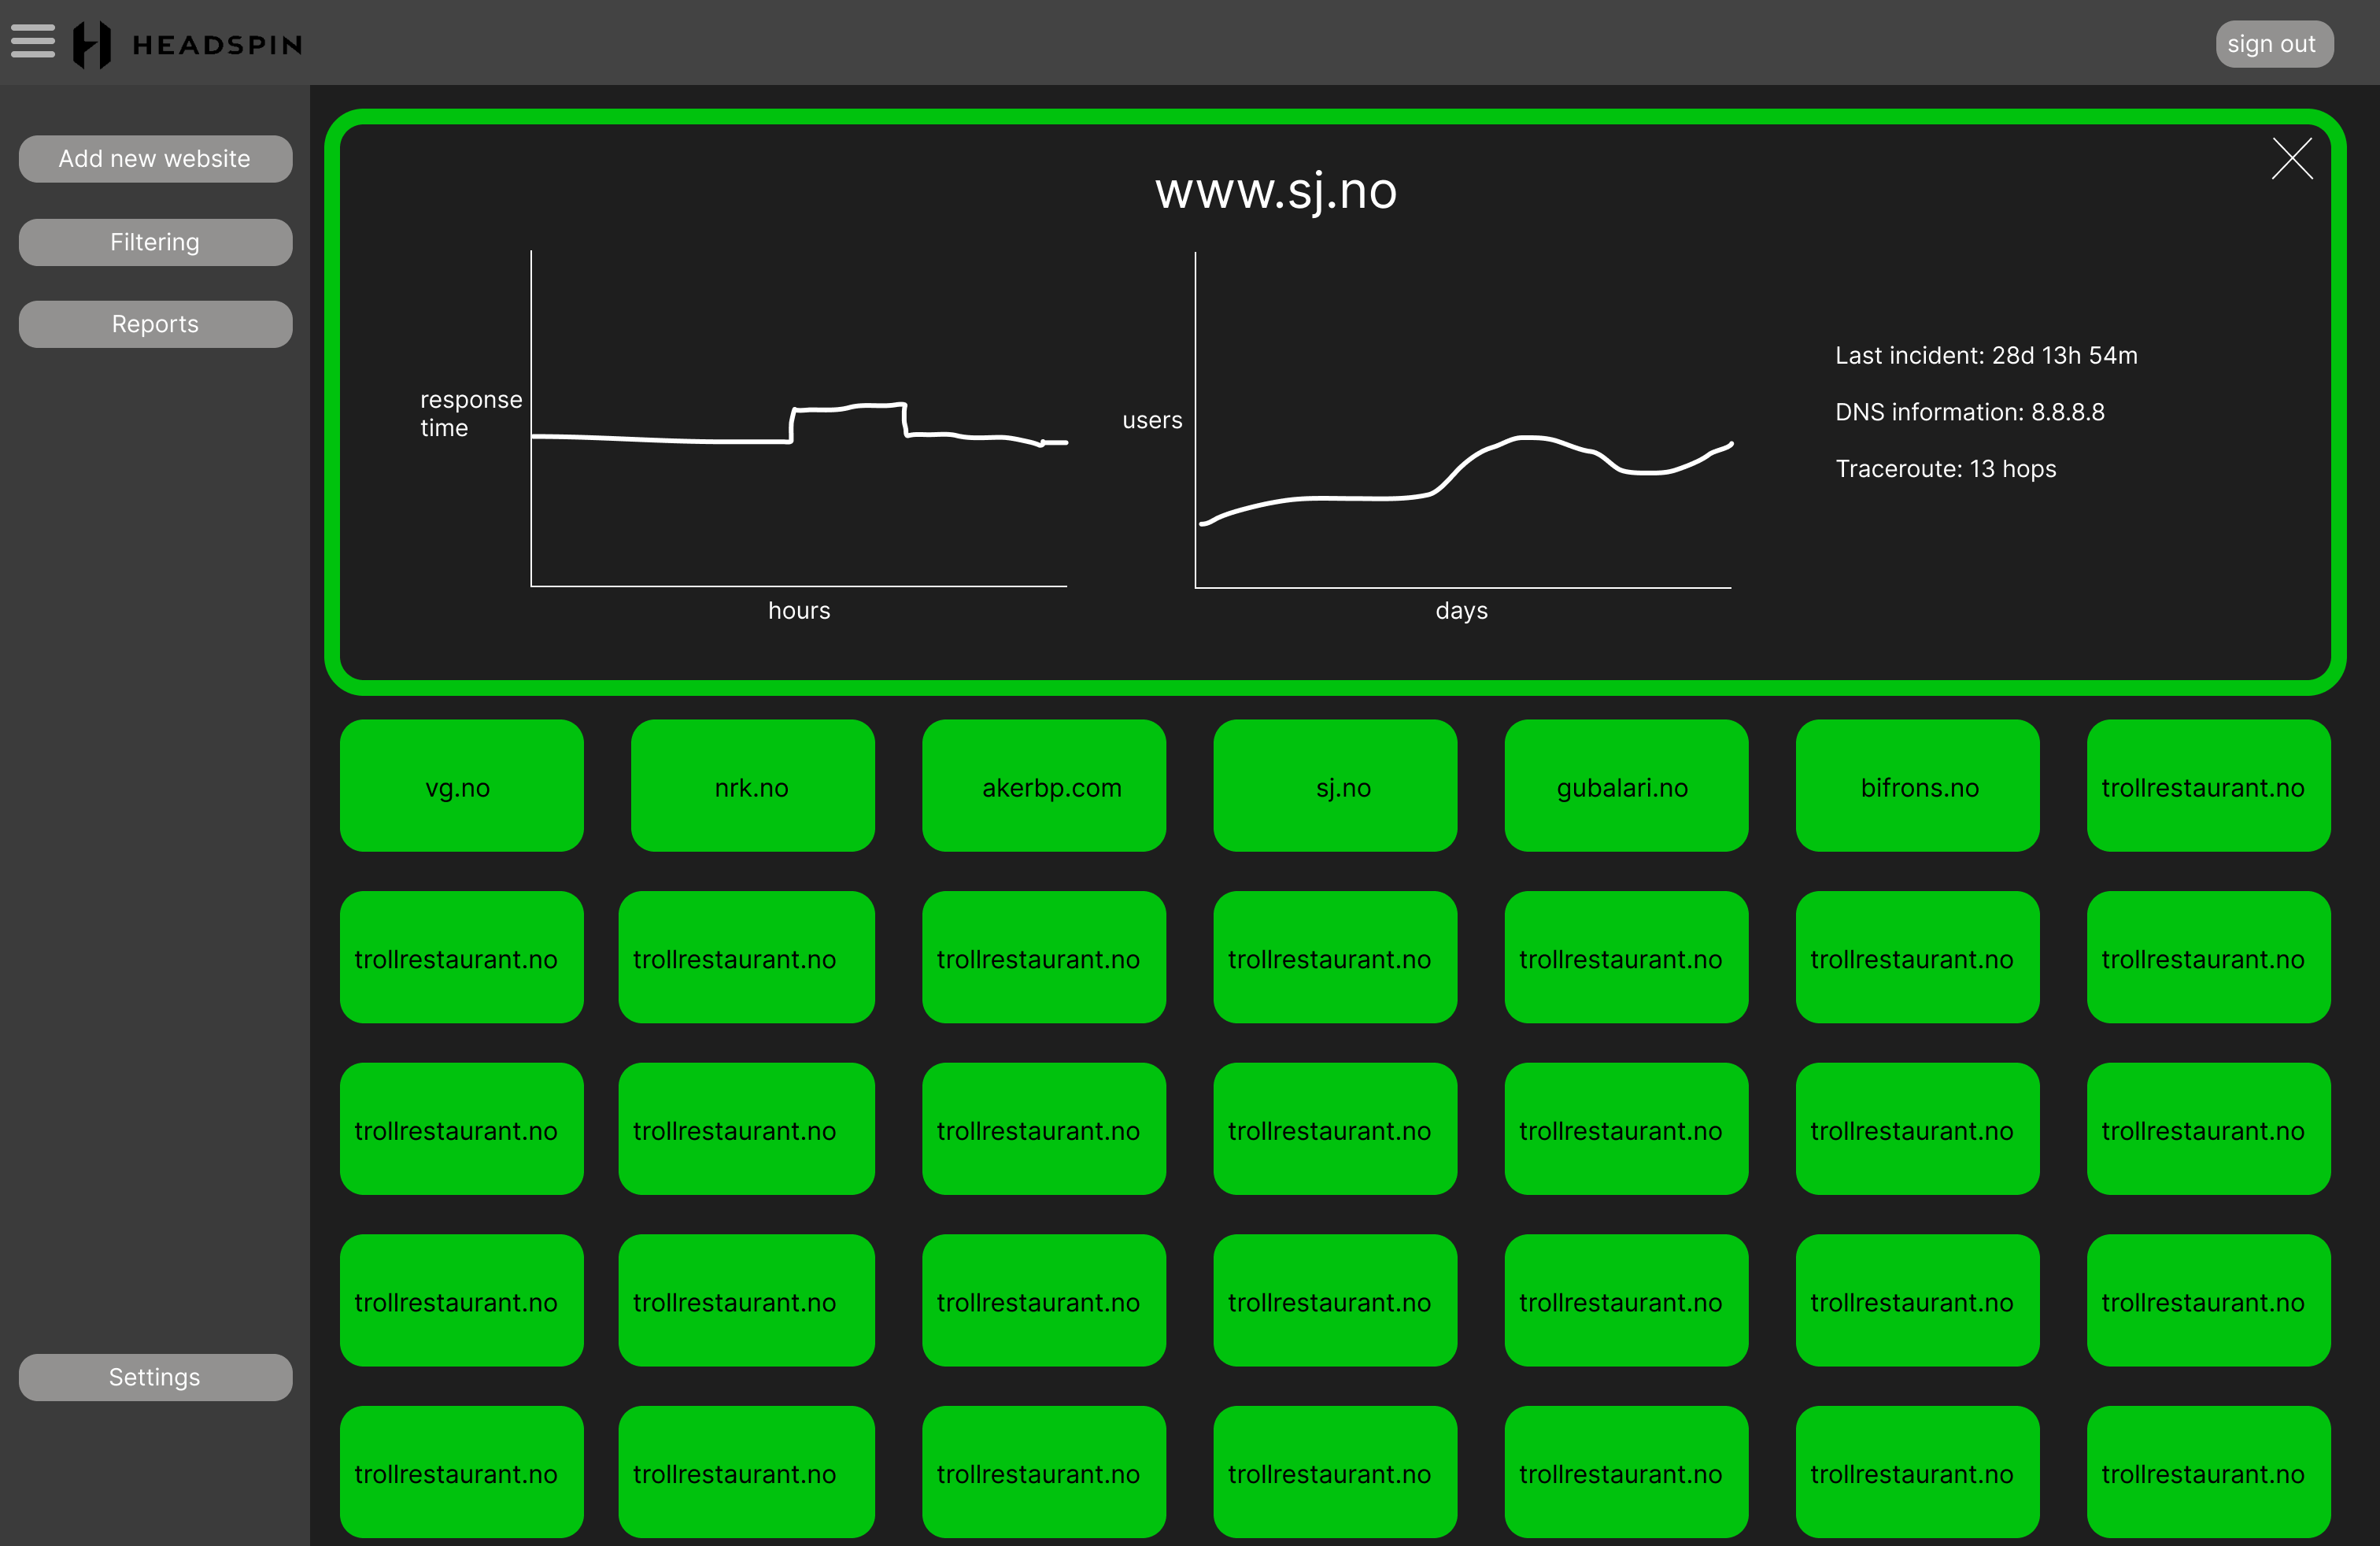
\includegraphics[width=1\linewidth]{figures/prototype_dashboard.png}
    \caption{Prototype of monitoring dashboard}
    \label{fig:proto_dash}
\end{figure}



\subsection{Refined Requirements for Development}
\label{subsec:reqs_after_proto}

The insights gathered from both the stakeholder clarification meeting and \textbf{\hyperref[subsec:user_testing]{user test 1}} were consolidated into a refined set of functional and non-functional requirements.  One important design element that changed after the prototype was that we moved away from completely green or red cards on the dashboard, to instead display status in a more visually appealing way. This is what eventually resulted in the final design for the website cards (see \ref{subsubsec:website_card_design}). The following tables present the requirements used throughout the development phase to guide implementation, prioritize features, and support evaluation.


\begin{table}[H]
    \centering
    \caption{Refined Functional Requirements}
    \label{tab:functional_reqs_refined}
    \begin{tabular}{|c|>{\raggedright\arraybackslash}p{0.75\linewidth}|c|}
        \hline
        \textbf{Req ID} & \textbf{Requirement Title} & \textbf{Priority} \\
        \hline
        F.1 & Add, edit, and delete monitored websites via the GUI. & High \\
        \hline
        F.2 & Perform automated checks for up/down status. & High \\
        \hline
        F.3 & Display HTTP status, response time, and uptime history. & High \\
        \hline
        F.4 & Highlight down websites prominently. & High \\
        \hline
        F.5 & Implement user authentication with personalized dashboards. & Medium \\
        \hline
        F.6 & Send alerts via email or SMS. & Medium \\
        \hline
        F.7 & Provide filtering, sorting, and search options. & Medium \\
        \hline
        F.8 & Allow users to define alert thresholds. & Medium \\
        \hline
        F.9 & Let users change check intervals per site. & Medium \\
        \hline
        F.10 & Configure alert destination per website (e.g., email). & Low \\
        \hline
    \end{tabular}
\end{table}

\begin{table}[H]
    \centering
    \caption{Refined Non-Functional Requirements}
    \label{tab:nonfunctional_reqs_refined}
    \begin{tabular}{|c|>{\raggedright\arraybackslash}p{0.75\linewidth}|c|}
        \hline
        \textbf{Req ID} & \textbf{Requirement Title} & \textbf{Priority} \\
        \hline
        NF.1 & Dashboard data must be fresh and updated in near real-time. & High \\
        \hline
        NF.2 & Interface must highlight changes in website status clearly. & High \\
        \hline
        NF.3 & Support monitoring of at least 50 websites without lag. & Medium \\
        \hline
        NF.4 & Ensure maintainability and clear documentation. & Medium \\
        \hline
        NF.5 & Interface should be responsive across screen sizes. & Low \\
        \hline
    \end{tabular}
\end{table}

These refined requirements provided a reference point throughout development and testing. They reflect both stakeholder needs and user-centered refinements gathered from direct testing.

\subsection{Requirement Prioritization Process}
\label{subsec:req_prio_process}

To structure development efficiently, requirements were prioritized based on their impact on usability and project feasibility. High-priority features such as monitoring (F.1–F.4) and real-time updates (NF.1) were implemented first to provide core functionality early. Medium-priority features, including user authentication (F.5) and alert customization (F.8), were added in later iterations. Low-priority requirements, such as per-website email customization (F.10) and varied screen-size responsiveness (NF.5), were addressed as time allowed.